\documentclass[a4paper, 10pt, twoside]{article}
\usepackage[left=2cm, right=2cm, top=2cm, bottom=3cm]{geometry}
\usepackage[super]{natbib}
\usepackage{amsmath}
\usepackage[shortlabels]{enumitem}
\usepackage{bbold}
\usepackage{graphicx}
\usepackage{url}
\usepackage{hyperref}
\hypersetup{
    colorlinks=true,
    linkcolor=blue,
    filecolor=magenta,      
    urlcolor=cyan,
}


\begin{document}

\title{High Performance Computing - Micro Aevol}
\author{T\'eo Bouvard}
\maketitle

\section{Introduction}

\section{Version CPU}

\subsection{Analyse}

Afin de se familiariser avec le code, il est intéressant de profiler son exécution. Cela permet d'identifier la structure globale du programme ainsi que son chemin critique. Dans le cas d'Aevol, on remarque que la fonction \textit{run\_a\_step} est exécutée pour chaque pas de temps, dont le nombre d'itérations est spécifié par l'argument \textit{n\_steps}.
Dans cette fonction, les différentes étapes du modèle biologique sont exécutées successivement pour chaque organisme.

\subsubsection*{Parallélisation du modèle}

Toutes les étapes de ce modèle sont indépendantes pour chaque organisme sauf l'étape de sélection qui requiert la lecture de l'état des organismes voisins sur la grille. Une optimisation naturelle est donc de paralléliser le traitement de chaque organisme\label{parallel/orga}.

\subsubsection*{Latence du disque}

Une autre simple optimisation est de limiter les appels à \textit{printf}, qui ralentissent l'exécution de manière significative lorsque ces derniers sont très fréquents. En effet, en utilisant les arguments par défaut on diminue de moitié le temps d'exécution en redirigeant la sortie standard ainsi que la sortie d'erreur vers \textit{/dev/null}. Bien évidemment, cette optimisation n'est pas aussi significative lorsque l'on utilise des tailles de problèmes plus élevée, mais il est sage d'éviter des appels systèmes coûteux lorsqu'ils ne sont pas nécessaires. Une alternative à la redirection des stream serait d'ajouter un argument permettant de contrôler la verbosité du programme, et ainsi s'affranchir du coût de tous ces appels systèmes lors d'une exécution en mode silencieux.

De manière similaire, les écritures dans les fichiers de statistiques invoquant \textit{std::endl} ou \textit{std::flush} imposent la synchronisation des flux de sortie, ce qui peut avoir un coût d'appel système assez élevé lié à la lenteur de l'écriture sur disque. Une meilleure solution serait de stocker les statistiques en mémoire jusqu'au point de backup afin de les écrire dans des fichiers en batch, ce qui améliorerait le buffering déja proposé par l'OS.

\subsection{Implémentation}

Dans l'optique de mesurer uniquement l'optimisation des calculs du modèle biologique, les benchmarks qui suivent n'incluent pas le temps d'écriture des fichiers de backup. En effet, cette écriture est réalisée par un seul thread et peut nécéssiter la compression DEFLATE de plusieurs Go de données, ce qui influe de manière significative sur le temps d'exécution du programme. Cependant, c'est un coût qui n'est pas directement lié au modèle biologique que l'on cherche à optimiser, et qui n'est effectué qu'à chaque point de backup.

\hyperref[parallel/orga]{Parallélisation du cycle d'évolution}

\begin{figure}
	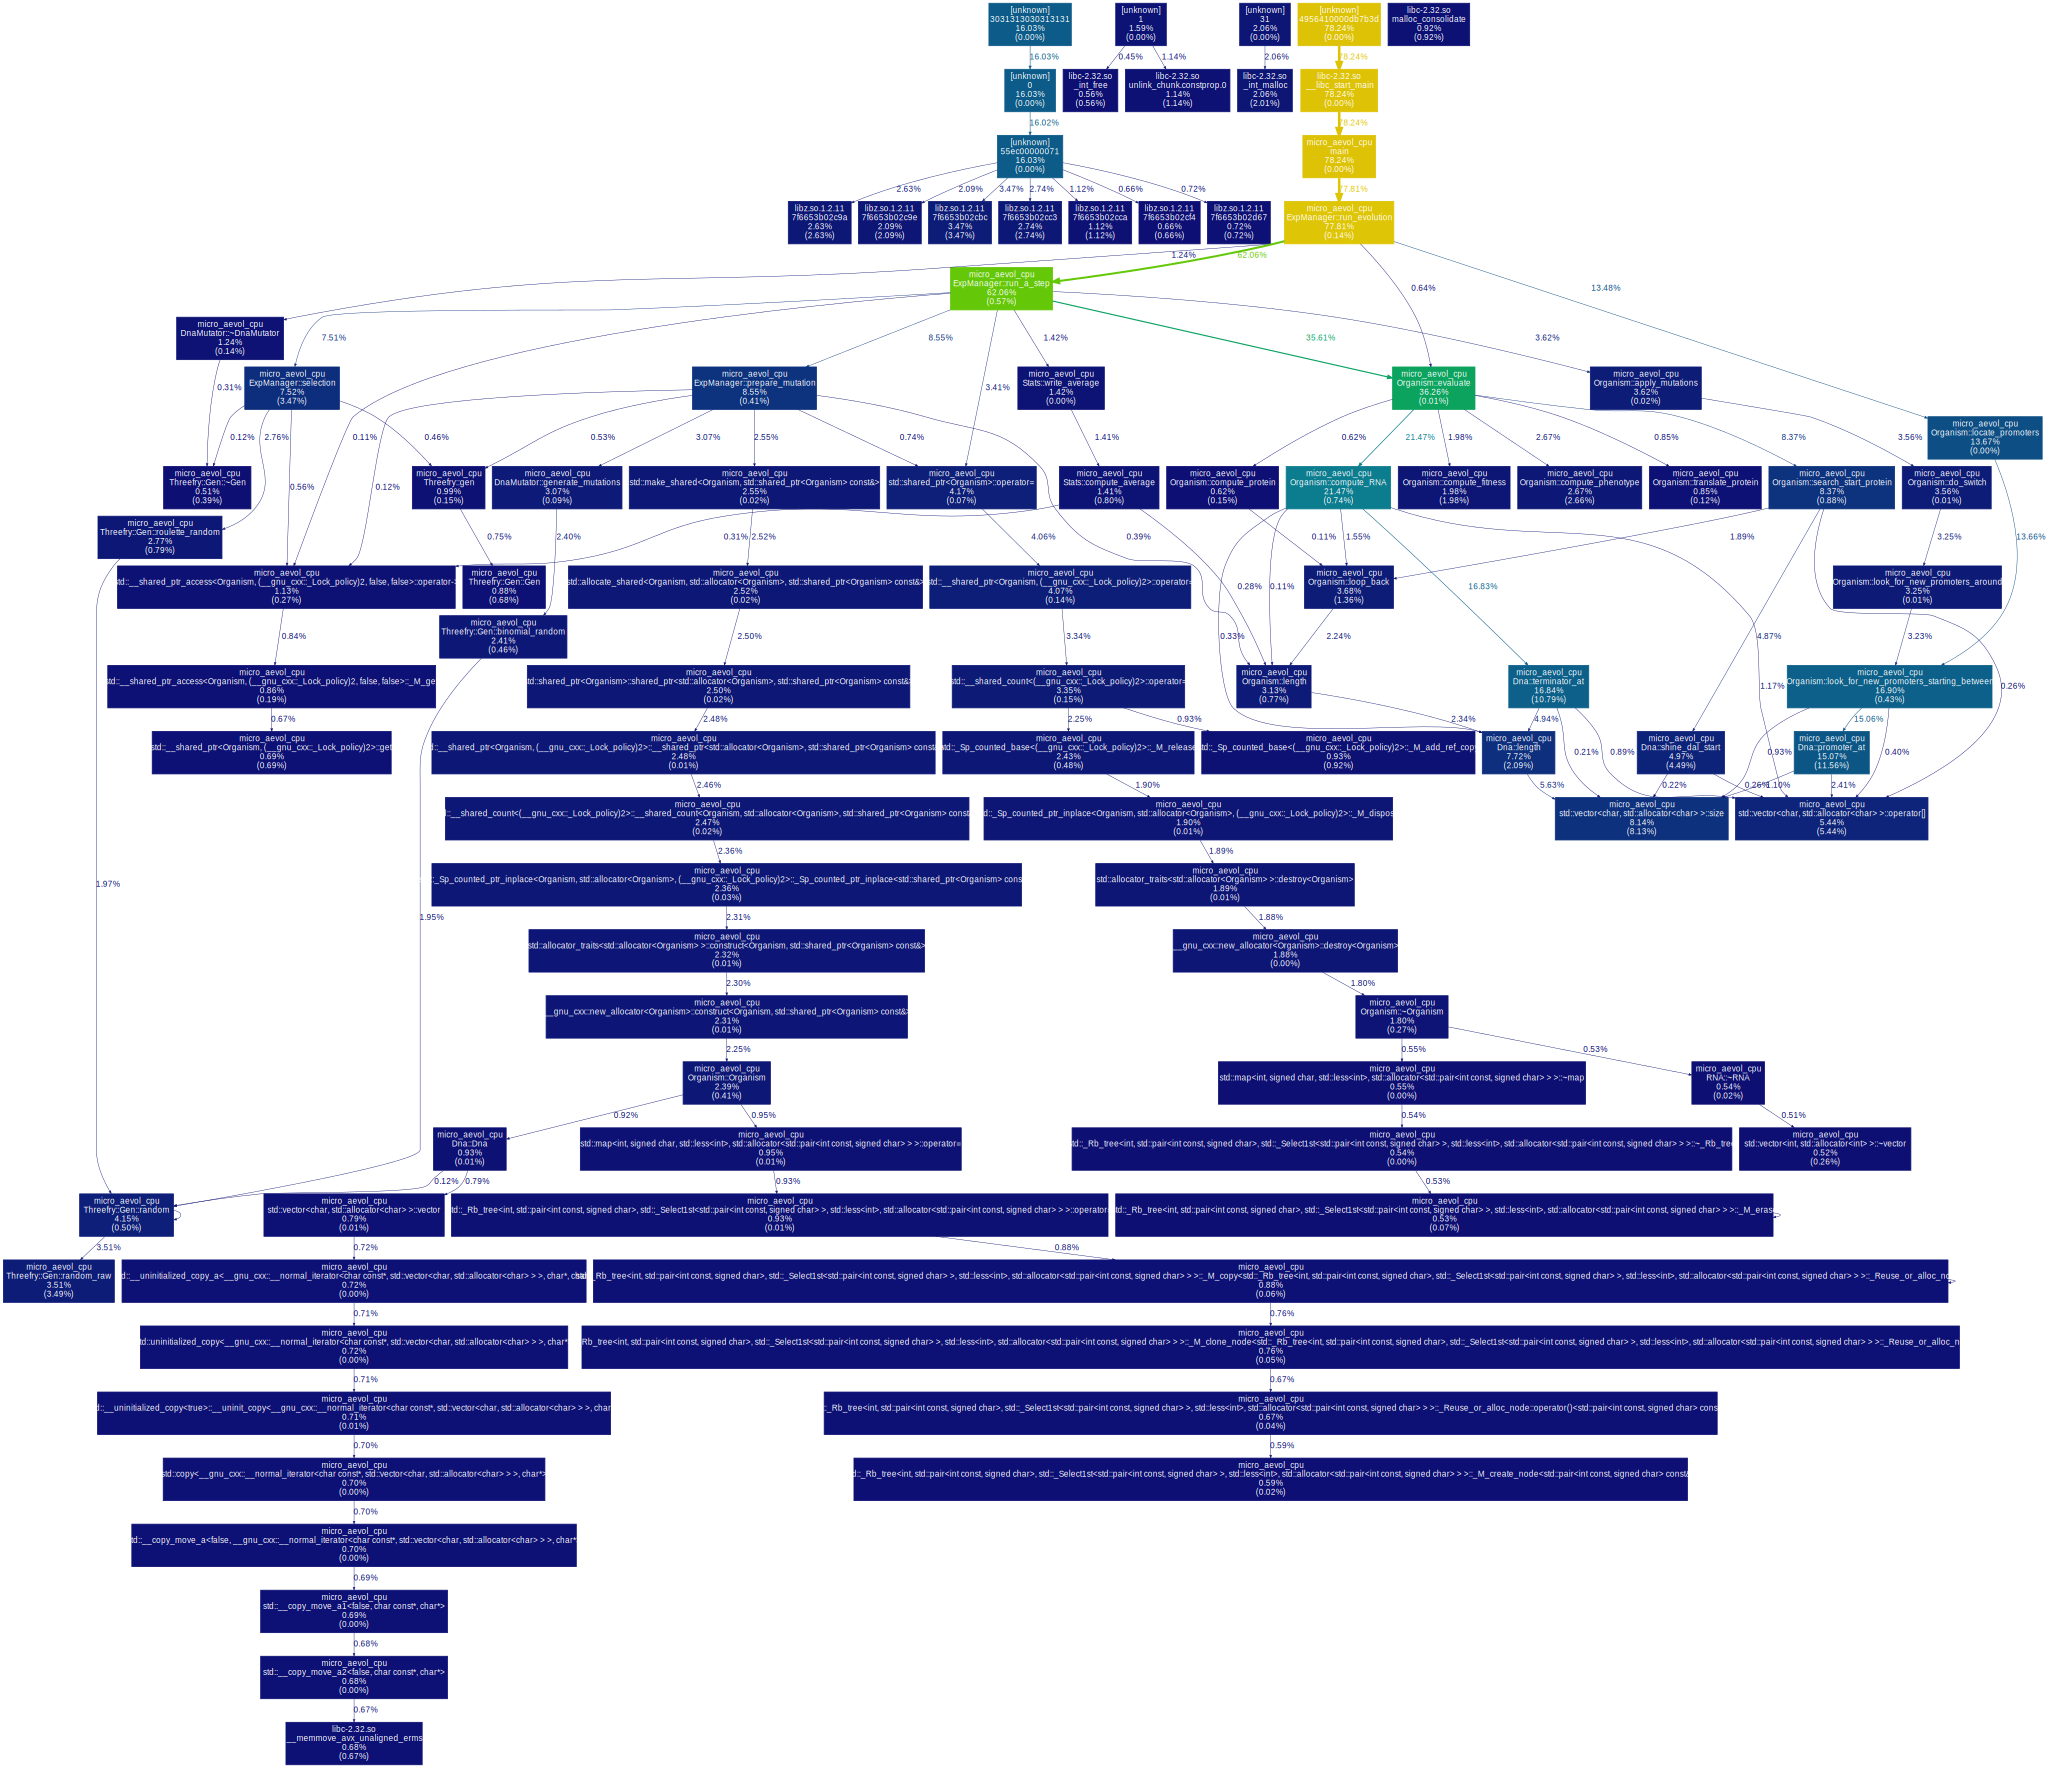
\includegraphics[width=\linewidth]{img/init_profile_debug.png}
\end{figure}
\section{Version GPU}

Divergence \citep{nvidia/branching}



\bibliographystyle{unsrtnat}
\bibliography{report}

\end{document}
